%---------------
%╔═╗╔═╗╔╦╗╦ ╦╔═╗
%╚═╗║╣  ║ ║ ║╠═╝
%╚═╝╚═╝ ╩ ╚═╝╩  
%---------------
\documentclass[12pt,oneside,a4paper]{report}

% DOCUMENT SETUP
\usepackage[left=3cm, 
			right=2.5cm, 
			top=2.5cm, 
			bottom=2.5cm, 
			includehead, 
			includefoot]{geometry}

% line spacing
\usepackage{setspace}
\setstretch{1,25} % 15/12 --> 1.25

%de­fines Adobe Times Ro­man as de­fault text font
\usepackage{mathptmx}
\usepackage{times} % needed for acronym package

%PDF linking package
\usepackage[hidelinks]{hyperref}

% Language Setup
\usepackage[ngerman]{babel}
% language specific bibliography style
\usepackage[numbers]{natbib}
\usepackage[fixlanguage]{babelbib}
\selectbiblanguage{german}
% bliographystyle setup
% default style names: apalike alphadin ieeetr IEEEtranSN apalike2 alphadin 
% babel specific: babplain, babplai3, babalpha, babunsrt, bababbrv, bababbr3 unsrt 
\bibliographystyle{unsrturl}

% encoding setup
% T1 font encoding for languages that use a latin alphabet
\usepackage[T1]{fontenc} 

% enhanced input encoding handling - utf8 for äÄüÜöÖß...
\usepackage[utf8]{inputenc}
%\usepackage{ucs}%utf8x suppart

% after babel - set chapter string
\AtBeginDocument{\renewcommand{\chaptername}{}}

% enumeration
\usepackage{enumitem}
% tabular extension tabularx
\usepackage{tabularx}

% math packages
\usepackage{amsmath}
\usepackage{nicefrac}
\usepackage{amsthm}
\usepackage{amsbsy}
\usepackage{amssymb}
\usepackage{amsfonts}
\usepackage{MnSymbol}

% patches for latex
\usepackage{fixltx2e}

%special characters
\usepackage{amssymb}
\usepackage{upgreek,textgreek}

% acronym package
\usepackage[printonlyused, footnote]{acronym}

% breakable text in \seqsplit{}
\usepackage{seqsplit}

% \textmu
\usepackage{textcomp}

% package provides a way to compile sections of a document using the same preamble as the main document
\usepackage{subfiles}

% driver-independent color extension - used by listings,tabularx
\usepackage[usenames,dvipsnames,table,xcdraw]{xcolor}

% -- SYNTAX HIGHLIGHTING --
\usepackage{listings}
%% bash command line Syntax Highlighting
\lstdefinestyle{BASH_CMD}{ 
  columns=fullflexible,            % copy pasteable listings
  language=bash,
  basicstyle=\small\sffamily,
  basicstyle   = \small \ttfamily,
  keywordstyle = [1]\small \ttfamily,
  keywordstyle = [2]\small \ttfamily,
  commentstyle = \small \ttfamily,
  numbers=none,
  captionpos=b, 
  breaklines=true,
  numberstyle=\tiny,
  numbersep=3pt,
  frame=tlrb,
  columns=fullflexible,
  backgroundcolor=\color{white!20},
  linewidth=\linewidth,
  literate=                        % replace in code
     {Ö}{{\"O}}1
     {Ä}{{\"A}}1
     {Ü}{{\"U}}1
     {ß}{{\ss}}2
     {ü}{{\"u}}1
     {ä}{{\"a}}1
     {ö}{{\"o}}1
}
 % adds style BASH_CMD
%% Matlab Syntax Highlighting
\colorlet{keyword}{blue!100!black!80}
\colorlet{STD}{Lavender}
\colorlet{comment}{green!90!black!90}
\definecolor{mygreen}{rgb}{0,0.6,0}
\definecolor{mygray}{rgb}{0.5,0.5,0.5}
\definecolor{mymauve}{rgb}{0.58,0,0.82}


\lstdefinestyle{BASH_SCRIPT}{ 
  language     = bash,
  basicstyle   = \footnotesize \ttfamily,
  keywordstyle = [1]\color{keyword}\bfseries,
  keywordstyle = [2]\color{STD}\bfseries,
  commentstyle = \color{mygreen}\itshape,
  backgroundcolor=\color{white},   % choose the background color; you must add \usepackage{color} 
  columns=fullflexible,            % copy pasteable listings
                                   % or \usepackage{xcolor}
  basicstyle=\footnotesize,        % the size of the fonts that are used for the code
  breakatwhitespace=false,         % sets if automatic breaks should only happen at whitespace
  breaklines=true,                 % sets automatic line breaking
  captionpos=b,                    % sets the caption-position to bottom
  extendedchars=true,              % lets you use non-ASCII characters; for 8-bits encodings only,
                                   % does not work with UTF-8
  frame=single,                    % adds a frame around the code
  keepspaces=true,                 % keeps spaces in text, useful for keeping indentation of code
                                   % (possibly needs columns=flexible)
  numbers=left,                    % where to put the line-numbers; possible values are 
                                   % (none, left, right)
  numbersep=5pt,                   % how far the line-numbers are from the code
  numberstyle=\tiny\color{mygray}, % the style that is used for the line-numbers
  rulecolor=\color{black},         % if not set, the frame-color may be changed on line-breaks
                                   % within not-black text (e.g. comments (green here))
  showspaces=false,                % show spaces everywhere adding particular underscores; it
  	                               % overrides 'showstringspaces'
  showstringspaces=false,          % underline spaces within strings only
  showtabs=false,                  % show tabs within strings adding particular underscores
  stepnumber=1,                    % the step between two line-numbers. If it's 1, each line 
                                   % will be numbered
  stringstyle=\color{mymauve},     % string literal style
  tabsize=2,                       % sets default tabsize to 2 spaces
  title=\lstname,                  % set title name
  literate=                        % replace in code
     {Ö}{{\"O}}1
     {Ä}{{\"A}}1
     {Ü}{{\"U}}1
     {ß}{{\ss}}2
     {ü}{{\"u}}1
     {ä}{{\"a}}1
     {ö}{{\"o}}1
} % adds style BASH_SCRIPT
% Matlab Syntax Highlighting
\colorlet{keyword}{blue!100!black!80}
\colorlet{STD}{red}
\colorlet{comment}{green!90!black!90}
\definecolor{mygreen}{rgb}{0,0.6,0}
\definecolor{mygray}{rgb}{0.5,0.5,0.5}
\definecolor{mymauve}{rgb}{0.58,0,0.82}


\lstdefinestyle{LATEX}{ 
  language     = [LaTeX]{TeX},
  basicstyle   = \footnotesize \ttfamily,
  keywordstyle = [1]\color{keyword}\bfseries,
  keywordstyle = [2]\color{comment}\bfseries,
  commentstyle = \color{mygray}\itshape,
  %backgroundcolor=\color{white},   % choose the background color; you must add \usepackage{color} 
                                   % or \usepackage{xcolor}
  basicstyle=\footnotesize,        		   % the size of the fonts that are used for the code
  breakatwhitespace=false,         % sets if automatic breaks should only happen at whitespace
  columns=fullflexible,            % copy pasteable listings
  breaklines=true,                 % sets automatic line breaking
  captionpos=c,                    % sets the caption-position to bottom
  extendedchars=true,              % lets you use non-ASCII characters; for 8-bits encodings only,
                                   % does not work with UTF-8
  frame=single,                    % adds a frame around the code
  keepspaces=true,                 % keeps spaces in text, useful for keeping indentation of code
                                   % (possibly needs columns=flexible)
  numbers=left,                    % where to put the line-numbers; possible values are 
                                   % (none, left, right)
  numbersep=4pt,                   % how far the line-numbers are from the code
  numberstyle=\tiny\color{mygray}, % the style that is used for the line-numbers
  rulecolor=\color{black},         % if not set, the frame-color may be changed on line-breaks
                                   % within not-black text (e.g. comments (green here))
  showspaces=false,                % show spaces everywhere adding particular underscores; it
  	                               % overrides 'showstringspaces'
  showstringspaces=false,          % underline spaces within strings only
  showtabs=false,                  % show tabs within strings adding particular underscores
  stepnumber=1,                    % the step between two line-numbers. If it's 1, each line 
                                   % will be numbered
  stringstyle=\color{mymauve},     % string literal style
  tabsize=2,                       % sets default tabsize to 2 spaces
  title=\lstname,                  % set title name
  literate=                        % replace in code
     {Ö}{{\"O}}1
     {Ä}{{\"A}}1
     {Ü}{{\"U}}1
     {ß}{{\ss}}2
     {ü}{{\"u}}1
     {ä}{{\"a}}1
     {ö}{{\"o}}1
} % adds style LATEX
%% Matlab Syntax Highlighting
\colorlet{keyword}{blue!100!black!80}
\colorlet{STD}{Lavender}
\colorlet{comment}{green!90!black!90}
\definecolor{mygreen}{rgb}{0,0.6,0}
\definecolor{mygray}{rgb}{0.5,0.5,0.5}
\definecolor{mymauve}{rgb}{0.58,0,0.82}


\lstdefinestyle{MATLAB}{ 
  language     = Matlab,
  basicstyle   = \footnotesize \ttfamily,
  keywordstyle = [1]\color{keyword}\bfseries,
  keywordstyle = [2]\color{STD}\bfseries,
  commentstyle = \color{mygreen}\itshape,
  backgroundcolor=\color{white},   % choose the background color; you must add \usepackage{color} 
                                   % or \usepackage{xcolor}
  basicstyle=\footnotesize,        % the size of the fonts that are used for the code
  breakatwhitespace=false,         % sets if automatic breaks should only happen at whitespace
  columns=fullflexible,            % copy pasteable listings
  breaklines=false,                % sets automatic line breaking
  captionpos=c,                    % sets the caption-position to bottom
  extendedchars=true,              % lets you use non-ASCII characters; for 8-bits encodings only,
                                   % does not work with UTF-8
  frame=single,                    % adds a frame around the code
  keepspaces=true,                 % keeps spaces in text, useful for keeping indentation of code
                                   % (possibly needs columns=flexible)
  numbers=left,                    % where to put the line-numbers; possible values are 
                                   % (none, left, right)
  numbersep=5pt,                   % how far the line-numbers are from the code
  numberstyle=\tiny\color{mygray}, % the style that is used for the line-numbers
  rulecolor=\color{black},         % if not set, the frame-color may be changed on line-breaks
                                   % within not-black text (e.g. comments (green here))
  showspaces=false,                % show spaces everywhere adding particular underscores; it
  	                               % overrides 'showstringspaces'
  showstringspaces=false,          % underline spaces within strings only
  showtabs=false,                  % show tabs within strings adding particular underscores
  stepnumber=1,                    % the step between two line-numbers. If it's 1, each line 
                                   % will be numbered
  stringstyle=\color{mymauve},     % string literal style
  tabsize=2,                       % sets default tabsize to 2 spaces
  title=\lstname,                  % set title name
  literate=                        % replace in code
     {Ö}{{\"O}}1
     {Ä}{{\"A}}1
     {Ü}{{\"U}}1
     {ß}{{\ss}}2
     {ü}{{\"u}}1
     {ä}{{\"a}}1
     {ö}{{\"o}}1
} % adds style MATLAB
% Matlab Syntax Highlighting
\colorlet{keyword}{blue!100!black!80}
\colorlet{STD}{Lavender}
\colorlet{comment}{green!90!black!90}
\definecolor{mygreen}{rgb}{0,0.6,0}
\definecolor{mygray}{rgb}{0.5,0.5,0.5}
\definecolor{mymauve}{rgb}{0.58,0,0.82}


\lstdefinestyle{PYTHON}{ 
  language     = Python,
  basicstyle   = \footnotesize \ttfamily,
  keywordstyle = [1]\color{keyword}\bfseries,
  keywordstyle = [2]\color{STD}\bfseries,
  commentstyle = \color{mygreen}\itshape,
  backgroundcolor=\color{white},   % choose the background color; you must add \usepackage{color} 
                                   % or \usepackage{xcolor}
  basicstyle=\footnotesize,        % the size of the fonts that are used for the code
  columns=fullflexible,            % copy pasteable listings
  breakatwhitespace=false,         % sets if automatic breaks should only happen at whitespace
  breaklines=false,                % sets automatic line breaking
  captionpos=c,                    % sets the caption-position to bottom
  extendedchars=true,              % lets you use non-ASCII characters; for 8-bits encodings only,
                                   % does not work with UTF-8
  frame=single,                    % adds a frame around the code
  keepspaces=true,                 % keeps spaces in text, useful for keeping indentation of code
                                   % (possibly needs columns=flexible)
  numbers=left,                    % where to put the line-numbers; possible values are 
                                   % (none, left, right)
  numbersep=5pt,                   % how far the line-numbers are from the code
  numberstyle=\tiny\color{mygray}, % the style that is used for the line-numbers
  rulecolor=\color{black},         % if not set, the frame-color may be changed on line-breaks
                                   % within not-black text (e.g. comments (green here))
  showspaces=false,                % show spaces everywhere adding particular underscores; it
  	                               % overrides 'showstringspaces'
  showstringspaces=false,          % underline spaces within strings only
  showtabs=false,                  % show tabs within strings adding particular underscores
  stepnumber=1,                    % the step between two line-numbers. If it's 1, each line 
                                   % will be numbered
  stringstyle=\color{mymauve},     % string literal style
  tabsize=2,                       % sets default tabsize to 2 spaces
  title=\lstname,                  % set title name
  literate=                        % replace in code
     {Ö}{{\"O}}1
     {Ä}{{\"A}}1
     {Ü}{{\"U}}1
     {ß}{{\ss}}2
     {ü}{{\"u}}1
     {ä}{{\"a}}1
     {ö}{{\"o}}1
} % adds style PYTHON
%% Matlab Syntax Highlighting
\colorlet{keyword}{blue!100!black!80}
\colorlet{STD}{Lavender}
\colorlet{comment}{green!90!black!90}
\definecolor{mygreen}{rgb}{0,0.6,0}
\definecolor{mygray}{rgb}{0.5,0.5,0.5}
\definecolor{mymauve}{rgb}{0.58,0,0.82}


\lstdefinestyle{CPP}{ 
  language     = C++,
  basicstyle   = \footnotesize \ttfamily,
  keywordstyle = [1]\color{keyword}\bfseries,
  keywordstyle = [2]\color{STD}\bfseries,
  commentstyle = \color{mygreen}\itshape,
  backgroundcolor=\color{white},   % choose the background color; you must add \usepackage{color} 
                                   % or \usepackage{xcolor}
  columns=fullflexible,            % copy pasteable listings
  basicstyle=\footnotesize,        % the size of the fonts that are used for the code
  breakatwhitespace=false,         % sets if automatic breaks should only happen at whitespace
  breaklines=false,                % sets automatic line breaking
  captionpos=c,                    % sets the caption-position to bottom
  extendedchars=true,              % lets you use non-ASCII characters; for 8-bits encodings only,
                                   % does not work with UTF-8
  frame=single,                    % adds a frame around the code
  keepspaces=true,                 % keeps spaces in text, useful for keeping indentation of code
                                   % (possibly needs columns=flexible)
  numbers=left,                    % where to put the line-numbers; possible values are 
                                   % (none, left, right)
  numbersep=5pt,                   % how far the line-numbers are from the code
  numberstyle=\tiny\color{mygray}, % the style that is used for the line-numbers
  rulecolor=\color{black},         % if not set, the frame-color may be changed on line-breaks
                                   % within not-black text (e.g. comments (green here))
  showspaces=false,                % show spaces everywhere adding particular underscores; it
  	                               % overrides 'showstringspaces'
  showstringspaces=false,          % underline spaces within strings only
  showtabs=false,                  % show tabs within strings adding particular underscores
  stepnumber=1,                    % the step between two line-numbers. If it's 1, each line 
                                   % will be numbered
  stringstyle=\color{mymauve},     % string literal style
  tabsize=2,                       % sets default tabsize to 2 spaces
  title=\lstname,                  % set title name
  literate=                        % replace in code
     {Ö}{{\"O}}1
     {Ä}{{\"A}}1
     {Ü}{{\"U}}1
     {ß}{{\ss}}2
     {ü}{{\"u}}1
     {ä}{{\"a}}1
     {ö}{{\"o}}1
} % adds style CPP
%% Matlab Syntax Highlighting
\colorlet{keyword}{blue!100!black!80}
\colorlet{STD}{Lavender}
\colorlet{comment}{green!90!black!90}
\definecolor{mygreen}{rgb}{0,0.6,0}
\definecolor{mygray}{rgb}{0.5,0.5,0.5}
\definecolor{mymauve}{rgb}{0.58,0,0.82}


\lstdefinestyle{C}{ 
  language     = C,
  basicstyle   = \footnotesize \ttfamily,
  keywordstyle = [1]\color{keyword}\bfseries,
  keywordstyle = [2]\color{STD}\bfseries,
  commentstyle = \color{mygreen}\itshape,
  backgroundcolor=\color{white},   % choose the background color; you must add \usepackage{color} 
  columns=fullflexible,            % copy pasteable listings
                                   % or \usepackage{xcolor}
  basicstyle=\footnotesize,        % the size of the fonts that are used for the code
  breakatwhitespace=false,         % sets if automatic breaks should only happen at whitespace
  breaklines=false,                % sets automatic line breaking
  captionpos=c,                    % sets the caption-position to bottom
  extendedchars=true,              % lets you use non-ASCII characters; for 8-bits encodings only,
                                   % does not work with UTF-8
  frame=single,                    % adds a frame around the code
  keepspaces=true,                 % keeps spaces in text, useful for keeping indentation of code
                                   % (possibly needs columns=flexible)
  numbers=left,                    % where to put the line-numbers; possible values are 
                                   % (none, left, right)
  numbersep=5pt,                   % how far the line-numbers are from the code
  numberstyle=\tiny\color{mygray}, % the style that is used for the line-numbers
  rulecolor=\color{black},         % if not set, the frame-color may be changed on line-breaks
                                   % within not-black text (e.g. comments (green here))
  showspaces=false,                % show spaces everywhere adding particular underscores; it
  	                               % overrides 'showstringspaces'
  showstringspaces=false,          % underline spaces within strings only
  showtabs=false,                  % show tabs within strings adding particular underscores
  stepnumber=1,                    % the step between two line-numbers. If it's 1, each line 
                                   % will be numbered
  stringstyle=\color{mymauve},     % string literal style
  tabsize=2,                       % sets default tabsize to 2 spaces
  title=\lstname,                  % set title name
  literate=                        % replace in code
     {Ö}{{\"O}}1
     {Ä}{{\"A}}1
     {Ü}{{\"U}}1
     {ß}{{\ss}}2
     {ü}{{\"u}}1
     {ä}{{\"a}}1
     {ö}{{\"o}}1
} % adds style C
%% JSON Syntax Highlighting
\colorlet{keyword}{blue!100!black!80}
\colorlet{STD}{Lavender}
\colorlet{comment}{green!90!black!90}
\definecolor{mygreen}{rgb}{0,0.6,0}
\definecolor{mygray}{rgb}{0.5,0.5,0.5}
\definecolor{mymauve}{rgb}{0.58,0,0.82}

\newcommand\JSONnumbervaluestyle{\color{blue}}
\newcommand\JSONstringvaluestyle{\color{red}}

\newif\ifcolonfoundonthisline

\makeatletter

\lstdefinelanguage{json}
{
  showstringspaces    = false,
  keywords            = {false,true},
  alsoletter          = 0123456789.,
  morestring          = [s]{"}{"},
  morestring          = [s]{'}{'},
  stringstyle         = \ifcolonfoundonthisline\JSONstringvaluestyle\fi,
  MoreSelectCharTable =%
    \lst@DefSaveDef{`:}\colon@json{\processColon@json},
  basicstyle          = \ttfamily,
  keywordstyle        = \ttfamily\bfseries,
}

% flip the switch if a colon is found in Pmode
\newcommand\processColon@json{
  \colon@json%
  \ifnum\lst@mode=\lst@Pmode%
    \global\colonfoundonthislinetrue%
  \fi
}

\lst@AddToHook{Output}{%
  \ifcolonfoundonthisline%
    \ifnum\lst@mode=\lst@Pmode%
      \def\lst@thestyle{\JSONnumbervaluestyle}%
    \fi
  \fi
  %override by keyword style if a keyword is detected!
  \lsthk@DetectKeywords% 
}

% reset the switch at the end of line
\lst@AddToHook{EOL}%
  {\global\colonfoundonthislinefalse}

\makeatother



\lstdefinestyle{JSON}{ 
  language     = json,
  basicstyle   = \footnotesize \ttfamily,
  keywordstyle = [1]\color{keyword}\bfseries,
  keywordstyle = [2]\color{STD}\bfseries,
  commentstyle = \color{mygreen}\itshape,
  backgroundcolor=\color{white},   % choose the background color; you must add \usepackage{color} 
                                   % or \usepackage{xcolor}
  basicstyle=\footnotesize,        % the size of the fonts that are used for the code
  columns=fullflexible,            % copy pasteable listings
  breakatwhitespace=false,         % sets if automatic breaks should only happen at whitespace
  breaklines=false,                % sets automatic line breaking
  captionpos=c,                    % sets the caption-position to bottom
  extendedchars=true,              % lets you use non-ASCII characters; for 8-bits encodings only,
                                   % does not work with UTF-8
  frame=single,                    % adds a frame around the code
  keepspaces=true,                 % keeps spaces in text, useful for keeping indentation of code
                                   % (possibly needs columns=flexible)
  numbers=left,                    % where to put the line-numbers; possible values are 
                                   % (none, left, right)
  numbersep=5pt,                   % how far the line-numbers are from the code
  numberstyle=\tiny\color{mygray}, % the style that is used for the line-numbers
  rulecolor=\color{black},         % if not set, the frame-color may be changed on line-breaks
                                   % within not-black text (e.g. comments (green here))
  showspaces=false,                % show spaces everywhere adding particular underscores; it
  	                               % overrides 'showstringspaces'
  showstringspaces=false,          % underline spaces within strings only
  showtabs=false,                  % show tabs within strings adding particular underscores
  stepnumber=1,                    % the step between two line-numbers. If it's 1, each line 
                                   % will be numbered
  stringstyle=\color{mymauve},     % string literal style
  tabsize=2,                       % sets default tabsize to 2 spaces
  title=\lstname,                  % set title name
  literate=                        % replace in code
     {Ö}{{\"O}}1
     {Ä}{{\"A}}1
     {Ü}{{\"U}}1
     {ß}{{\ss}}2
     {ü}{{\"u}}1
     {ä}{{\"a}}1
     {ö}{{\"o}}1
} % adds style JSON

% HEADLINE CFG
\usepackage{fancyhdr} % Headers and footers
\usepackage{lastpage}
\usepackage{nopageno}
\setlength{\headheight}{1.5cm}
\pagestyle{fancy} % All pages have headers and footers
\fancyhead{} % Blank out the default header
\fancyfoot{} % Blank out the default footer
\fancyhead[L]{}
\fancyhead[C]{}
\fancyhead[R]{}
\fancyfoot[L]{}
\fancyfoot[C]{\thepage}
\fancyfoot[R]{}
% override plain page style for \part, \chapter or 
% \maketitle, which implicit specifies plain page style
\fancypagestyle{plain} 
{
	\fancyhead[L]{}
	\fancyhead[C]{}
	\fancyhead[R]{}
	\fancyfoot[L]{}
	\fancyfoot[C]{\thepage}
	\fancyfoot[R]{}
}
% set list pagestyle
\fancypagestyle{lists} 
{
	\fancyhead[L]{}
	\fancyhead[C]{}
	\fancyhead[R]{}
	\fancyfoot[L]{}
	\fancyfoot[C]{\thepage}
	\fancyfoot[R]{}
}

\renewcommand{\chaptermark}[1]{\markright{#1}{}}
\renewcommand{\sectionmark}[1]{\markright{#1}{}}
\renewcommand{\headrulewidth}{0pt}
\renewcommand{\footrulewidth}{0pt}

	
\usepackage{verbatim}
\usepackage{graphicx}
\usepackage{epstopdf}

% floating prevention packages
\usepackage{float}    % used with [H] positioning parameter
\usepackage{placeins} % \FloatBarrier 

% tikz packages
\usepackage{tikz}
\usepackage{caption}
\usepackage[list=true,listformat=simple]{subcaption}
\usepackage{standalone}
\usepackage{pgfplots}


% include only specified tex files - uncommend unneeded
\includeonly{preface/cover,
             preface/abstract,
             preface/tableofcontents,
             preface/listoffigures,
             preface/listoftables,
             preface/lstlistoflistings,
             appendix/bibliography}

%-------------------
%╔═╗╔╦╗╦═╗╦╔╗╔╔═╗╔═╗
%╚═╗ ║ ╠╦╝║║║║║ ╦╚═╗
%╚═╝ ╩ ╩╚═╩╝╚╝╚═╝╚═╝
%-------------------
\newcommand{\strLecture}{Signale, Systeme und Sensoren}
\newcommand{\strDate}{\today}
\newcommand{\strAuthorA}{T. Gnädig}
\newcommand{\strAuthorB}{F. Gendusa}
\newcommand{\strAuthorAEmail}{thgnaedi@htwg-konstanz.de}
\newcommand{\strAuthorBEmail}{fagendus@htwg-konstanz.de}
% Versuchsbeschreibung 
\newcommand{\strTopic}{Kalibrierung und Einsatz einen Infrarot-Entfernungsmessers}
\newcommand{\strAbstract}{}
% hyperref customization
\hypersetup{
	pdftitle    ={\strTopic}, % title
	pdfsubject	={\strLecture}, % subject of the document
	pdfauthor	={\strAuthorA, \strAuthorB}, % author
	pdfkeywords	={}, % list of keywords
	pdfcreator	={}, % creator of the document
	pdfproducer	={}, % producer of the document
	colorlinks=false, % false: boxed links; true: colored links
	linkcolor=red, % color of internal links (change box color with linkbordercolor)
    citecolor=green, % color of links to bibliography
    filecolor=magenta, % color of file links
    urlcolor=cyan, % color of external links
	%bookmarks=true, % show bookmarks bar?
	unicode=true, % non-Latin characters in Acrobat’s bookmarks
	pdftoolbar=true, % show Acrobat’s toolbar?
	pdfmenubar=true, % show Acrobat’s menu?
    pdffitwindow=false, % window fit to page when opened
	pdfnewwindow=true % links in new PDF window
}

%-----------------------------------------
% ╔╗ ╔═╗╔═╗╦╔╗╔  ╔╦╗╔═╗╔═╗╦ ╦╔╦╗╔═╗╔╗╔╔╦╗ 
% ╠╩╗║╣ ║ ╦║║║║   ║║║ ║║  ║ ║║║║║╣ ║║║ ║  
% ╚═╝╚═╝╚═╝╩╝╚╝  ═╩╝╚═╝╚═╝╚═╝╩ ╩╚═╝╝╚╝ ╩  
%-----------------------------------------

\begin{document}
\pagenumbering{Roman} 

%\setcounter{section}{0}

\begin{titlepage}

\vspace*{-3.5cm}

\begin{flushleft}
\hspace*{-1cm} 

\includegraphics[width=15.7cm]{preface/htwg-logo}
\end{flushleft}

\vspace{1cm}

\begin{center}
	\large{
		\textbf{\strLecture} \\[2cm]
	}
	\Huge{
		\textbf{\strTopic} \\[2cm]
	}
	\Large{
		\textbf{\strAuthorA, \strAuthorB}} \\[3cm]
	\large{
		\textbf{} \\[2.3cm]
	}
	
	\large{
		\textbf{Konstanz, \strDate}
	}
\end{center}

\end{titlepage}
\thispagestyle{empty}




\begin{center}
{\Large \textbf{Zusammenfassung (Abstract)}}
\end{center}

\bigskip

\begin{center}
	\begin{tabular}{p{2.8cm}p{5cm}p{5cm}}
		Thema: & \multicolumn{2}{p{10cm}}{\raggedright\strTopic} \\
		 & & \\
		Autoren: & \strAuthorA & \href{mailto:\strAuthorAEmail}{\strAuthorAEmail} \\
		 & \strAuthorB & \href{mailto:\strAuthorBEmail}{\strAuthorBEmail} \\
		 & & \\
		Betreuer: & Prof. Dr. Matthias O. Franz & \href{mailto:mfranz@htwg-konstanz.de}{mfranz@htwg-konstanz.de} \\
		 &  Jürgen Keppler & \href{mailto:juergen.keppler@htwg-konstanz.de}{juergen.keppler@htwg-konstanz.de} \\
		 &  Martin Miller & \href{mailto:martin.miller@htwg-konstanz.de}{martin.miller@htwg-konstanz.de} \\
	\end{tabular}
\end{center}

\bigskip

\noindent
\strAbstract

\thispagestyle{lists}



\clearpage

%
% TABLE OF CONTENTS
%
\thispagestyle{lists}
%
% TABLE OF CONTENTS
%
\tableofcontents
\thispagestyle{plain}
\newpage

%
% Abbildungsverzeichnis
%
%
% Abbildungsverzeichnis
%
\phantomsection
\addcontentsline{toc}{chapter}{Abbildungsverzeichnis}
\listoffigures
\thispagestyle{lists}
\newpage

%
% Tabellenverzeichnis
%
%
% Tabellenverzeichnis
%
\phantomsection
\addcontentsline{toc}{chapter}{Tabellenverzeichnis}
\listoftables
\thispagestyle{lists}
\newpage

%
% Listingverzeichnis
%
%
% Listingverzeichnis
%
\phantomsection
\renewcommand\lstlistingname{Listing}
\renewcommand\lstlistlistingname{Listingverzeichnis}
\lstlistoflistings
\addcontentsline{toc}{chapter}{Listingverzeichnis}
\thispagestyle{lists}
\newpage


%--------------------------
% ╔═╗╦ ╦╔═╗╔═╗╔╦╗╔═╗╦═╗╔═╗ 
% ║  ╠═╣╠═╣╠═╝ ║ ║╣ ╠╦╝╚═╗ 
% ╚═╝╩ ╩╩ ╩╩   ╩ ╚═╝╩╚═╚═╝ 
%--------------------------

\pagenumbering{arabic} 
\setcounter{page}{1}
%
% CHAPTER Einleitung
%
\chapter{Einleitung}
\label{chap:EINL}
In diesem ersten Praktikum der Vorlesung Signale, Systeme und Sensoren beschäftigen wir uns mit einem Distanzsensor der Firma Sharp, welcher auch häufig in der Robotik Einsatz findet. Das Praktikum teilt sich in drei Aufgabenstellungen auf

\begin{itemize}
\item Bestimmen der Kennlinie des Sensors
\item Berechnen der Übertragungsfunktion(Kennline) mit Linearer Regression
\item Flächenberechnung eines DIN A4 Blattes und Fehlerberechnung
\end{itemize}

Bei dem verwendeten Abstandssensor handelt es sich um den SHARP \textit{GP2Y0A21YK0F}. Um den Sensor erfolgreich kalibrieren zu können \textit{(Umrechnungsvorschrift bestimmen)} finden ein Oszilloskop, sowie ein Meterstab als Bezugsnormal und eine reflektierende weiße Fläche Einsatz. Zur eigentlichen Bestimmung der Kennlinie wird die Lineare Regression eingesetzt.

Zur Verarbeitung der Messwerte wird die Programmiersprache Python eingesetzt. Die entsprechenden Listings sind an geeigneter Stelle referenziert.

%\cite{Franz2015j}    HAB ICH RAUSKOMMENTIERT

%
% CHAPTER Versuch 1
%
\chapter{Ermittlung der Sensorkennlinie}
\label{chap:VERSUCH_1}

\section{Fragestellung, Messprinzip, Aufbau, Messmittel}
\label{chap:VERSUCH_1_FRAGESTELLUNG}
In diesem ersten Teil werden wir die Kennlinie des Sensors ermitteln um für zukünftige Messungen mit diesem Senor einen Zusammenhang zwischen gemessenem Wert und eigentlicher Distanz \textit{(Sensor-Objekt)} zu haben. 
Dazu benutzen wir den bereits vorgestellten Sensor, ein Meterstab als Bezugsnormal, wie auch einer weißen Holzplatte als reflektierendes Objekt für den Infrarotstrahl des Sensors. Die Spannung am Output des Sensors wird mit einem Oszilloskop bestimmt. Dies ist zweckmäßig, da dieses an einem Computer angeschlossen werden kann und somit viele gemessene Spannungswerte eines Messvorgangs über die Zeit auf einfache weise abgespeichert werden können. 
\\
Um Distanzen zu bestimmen arbeitet der Sensor nach dem Triangulationsprinzip. Dieser aktive Sensor sendet einen Infrarotstrahl aus, welcher dann von einem Objekt reflektiert und schließlich von dem integrierten optischen Positionssensor und Signalprozessor in einen Spannungswert umgewandelt wird. Aufgrund der Abnahme des reflektierten Lichtes und den konstruktionsbedingten Eigenschaften des Sensors schränkt sich der Messbereich auf 10 -80 cm ein. Betrieben wird der Sensor mit einer Spannung von 5V.
Zum bestimmen der Sensorkennlinie wurden 20 verschiedene Abstandswerte im Bereich von 10 - 70 cm eingestellt, die als Werte für die Kalibrierung genügen müssen. Die Messwerte wurden mit einem Computer von dem Oszilloskop eingelesen \textit{(1500 Werte pro Distanz)}. Das $\Delta V$, sowie die durchschnittliche Spannung wurden vom Oszilloskop abgelesen. Das $\Delta V$ gibt die Breite des Rauschens an $\Delta V = U_{max} - U_{min}$ 
Zur Berechnung der Kennlinie jedoch werden die von dem Pythonscript \ref{chap:APPENDIX_SOURCECODE_V1} berechneten Mittelwerte $\bar{U}$ und $\Delta V$ der jeweils 1500 Messwerte benutzt. Zum Vergleich jedoch werden wir die handschriftlich ($hds$) entnommenen Werte auch tabellarisch darstellen. Tabelle \ref{tab:MESSWERTE1}. 

\section{Messwerte}
\begin{table}[H]
\centering
\begin{tabular}{cccccc}
\hline
Distanz in $cm$ & $\bar{U} $ in $V$ & $\Delta V$ in $V$ & $s_{\bar{x}}$ in $mV$ &  $\bar{U}_{\textit{hds}}$ in $V$ & $\Delta $V$_{\textit{hds}}$ in $V$\\ 
\hline  
 10.00 & 1.411 & 0.056 & 0.208 & 1.410 & 0.048\\
 13.15 & 1.296 & 0.04  & 0.177 & 1.250 & 0.048\\
 16.31 & 1.119 & 0.04  & 0.166 & 1.130 & 0.088\\
 19.47 & 1.013 & 0.08  & 0.453 & 1.010 & 0.080\\
 22.63 & 0.907 & 0.072 & 0.444 & 0.907 & 0.088\\
 25.79 & 0.820 & 0.068 & 0.430 & 0.820 & 0.076\\
 28.95 & 0.685 & 0.072 & 0.439 & 0.741 & 0.072\\
 32.10 & 0.635 & 0.068 & 0.392 & 0.682 & 0.068\\
 35.26 & 0.628 & 0.024 & 0.105 & 0.629 & 0.032\\
 38.42 & 0.587 & 0.024 & 0.105 & 0.588 & 0.032\\
 41.57 & 0.560 & 0.068 & 0.446 & 0.560 & 0.068\\
 44.74 & 0.540 & 0.068 & 0.444 & 0.540 & 0.072\\
 47.89 & 0.521 & 0.068 & 0.443 & 0.520 & 0.068\\
 51.05 & 0.481 & 0.072 & 0.444 & 0.501 & 0.068\\
 54.21 & 0.462 & 0.068 & 0.451 & 0.461 & 0.068\\
 57.37 & 0.442 & 0.072 & 0.448 & 0.441 & 0.072\\
 60.53 & 0.442 & 0.064 & 0.450 & 0.441 & 0.072\\
 63.68 & 0.422 & 0.068 & 0.447 & 0.422 & 0.068\\
 66.84 & 0.390 & 0.028 & 0.102 & 0.391 & 0.032\\
 70.00 & 0.390 & 0.024 & 0.098 & 0.391 & 0.024\\ 
 \hline
\end{tabular}
\caption{20 Messwerte aus Versuch 1}
\label{tab:MESSWERTE1}
\end{table}

\begin{figure}[H]
	\centering
	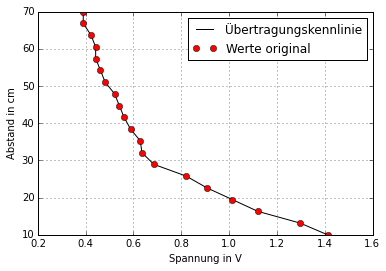
\includegraphics{media/durchschnittlicheMessergebnisse.png}
	\caption{Messwerte aus   \ref{tab:MESSWERTE1} $\bar{U}$  -  $\Delta V$}
	\label{img:MESSGRAFIK1}
\end{figure}
\section{Auswertung und Interpretation}
\label{chap:VERSUCH_1_AUSWERTUNG}
Bei Betrachtung der gemessenen Werte fällt zuerst auf, dass der Sensor ein umgekehrt proportionales Verhalten aufweist. So wird die Spannung $\bar{U}$ mit zunehmender Entfernung des Objektes kleiner. Die Differenzen der von dem Oszilloskop abgelesenen Werte und den berechneten Werten im Computer sind auf zwei verschiedene Ursachen zurückzuführen. Der Unterschied im Mittelwert, hängt mit dem Einschwingmoment des Sensors zusammen. Dieser wurde bei der Berechnung im Computer ausgelassen, da die ersten 1000 Messwerte übersprungen wurden. Der von dem Oszilloskop abgelesene Mittelwert jedoch beinhält den Einschwingmoment und hat somit eine geringere Genauigkeit als der im Computer berechnete.
Die Differenz im $\Delta V$ wird im wesentlichen durch das Einstellen des Cursors im Oszilloskop beeinflusst.
Daher zeichnet sich schon ab, dass die berechneten Werte im Computer genauer sein müssen, als die von dem Oszilloskop abgelesenen.
An Abbildung \ref{img:MESSGRAFIK1} sieht man, das es sich bei der Kennlinie des Sensors um eine Funktion handelt im Format $y = x^a$.
Dies ist auch nicht weiter verwunderlich, da die Intensität des Lichtes mit zunehmenden Abstand der Lichtquelle quadratisch abnimmt.
Da jede Messung nur einmal durchgeführt wurde ist zu bedenken, dass die Gefahr einer systematischen Unterschätzung des Messfehlers besteht.



%\section{Interpretation}
%\label{chap:VERSUCH_1_INTERPRETATION}

%
% CHAPTER Versuch 2
%
\chapter{Lineare Regression}
\label{chap:VERSUCH_2}

\section{Fragestellung, Messprinzip, Aufbau, Messmittel}
\label{chap:VERSUCH_2_FRAGESTELLUNG}
In diesem weiteren Teil unserer Versuchsreihe ermitteln wir nun eine Umrechnungsvorschrift für die gemessenen Spannungswerte und dem eigentlichen Abstand von Objekt zu Sensor.
Zur Bestimmung dieser Gleichung eignet sich die Lineare Regression.
Dabei wird davon ausgegangen, dass die Übertragungsfunktion linear ist und daher der Form $y = a \cdot x + b$ genügt. Zur Regression wird dann eine Ausgleichsgerade zwischen die Messpunkte gelegt. Dabei werden die quadrierten Abstände aller Datenpunkte und der Geraden minimiert. Dieser Vorgang wird in folgender Formel zum Ausdruck gebracht, wobei $E$ gerade die Summe der minimalen quadrierten Abstände, $a$ die Steigung \textit{(Sensitivität)} und $b$ der Geraden Offset darstellt.
\begin{equation}
 E = \sum_{i=1}^{n} (y_i - (a\cdot x_i + b))^2
\end{equation}
Da es sich bei der Kennlinie dieses Sensors nicht um eine lineare handelt, sondern um eine potenzielle $y = x^a$ \ref{chap:VERSUCH_1_AUSWERTUNG}, kann die Regression nicht direkt angewandt werden. Um dieses Problem zu lösen müssen die Wertpaare aus Teil 1 \ref{tab:MESSWERTE1} zuerst logarithmiert werden. Somit kommen die Werte in einen linearen Zusammenhang und können dann zur regression verwendet werden.
Nach dem Berechnen der Ausgleichsgeraden muss eine Rückrechnung erfolgen, damit der ursprüngliche Zusammenhang wieder hergestellt wird. Dies geschieht durch doppelte Logarithmierung:

\begin{equation}
y = exp(a \cdot \ln x \plus b) = e^b \cdot x^a
\end{equation}
\\
Die Konstanten $a$ und $b$ sind das Ergebnis der linearen Regression. Die Variable $x$ ist die Information, die der Sensor in Form einer Spannung bereitstellt und $y$ der korrespondierende Abstandswert in cm.
Berechnet wurden die Konstanten mit Hilfe eines Pythonscripts und der Bibliothek des Modules Numpy. Das entsprechenden Listings zur Logarithmierung und Regression sind im Anhang zu finden. \ref{chap:APPENDIX_SOURCECODE_V2} 
 
\section{Messwerte}
\label{chap:VERSUCH_2_MESSWERTE}
\begin{figure}[H]
    \centering
	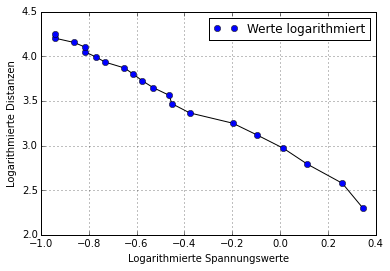
\includegraphics{media/LogaritmierteMessergebnisse.png}
	\caption{Logarithmierte Wertpaare}
	\label{img:LOGARITHMIERTE_WERTEPAARE}
\end{figure}

\begin{figure}[H]
    \centering
	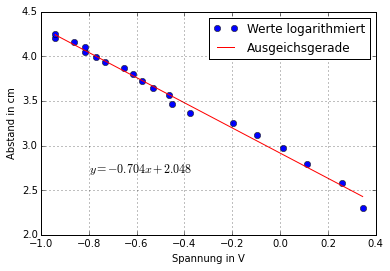
\includegraphics{media/LineareRegression.png}
	\caption{Lineare Regression}
	\label{img:LINEARE_REGRESSION}
\end{figure}
\begin{figure}[H]
    \centering
	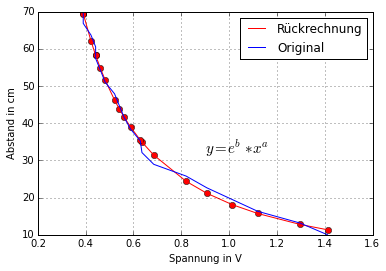
\includegraphics{media/vergleichOriginalLinreg.png}
	\caption{Rückrechnung und Ursprüngliche Messwerte}
	\label{img:RUECKRECHNUNG}
\end{figure}

\begin{table}[H]
\centering
\begin{tabular}{c|c}
 $a$ & -1.40898573049 \\ 
\hline $b$ & 2.91477669005 \\ 
\end{tabular} 
\caption{Ermittelte Konstanten der Linearen Regression und Rückrechnung}
\label{tab:KONSTANTEN_KENNLINIE}
\end{table}
\section{Auswertung und Interpretation}
\label{chap:VERSUCH_2_AUSWERTUNG}
In Abbildung \ref{img:LOGARITHMIERTE_WERTEPAARE} sind die Logarithmierten Wertpaare zu sehen. Dabei wurden die entsprechenden Spannungswerte auf der $x$-Achse aufgetragen und die dazugehörigen Distanzen auf die $y$-Achse.
Nun kann man die Lineare Regression anwenden. Das Resultat ist in Abbildung \ref{img:LINEARE_REGRESSION} zu sehen. Das Ergebnis der Rückrechnung auf den ursprünglichen Zusammenhang ist in Abbildung \ref{img:RUECKRECHNUNG} zu sehen. Rein optisch scheint die ermittelte Funktion relativ genau zu sein. Zum Vergleich ist die Kurve der originalen Messwerte auch mit aufgetragen(\textit{blau}). Als Umrechnungsvorschrift ergibt sich also folgende Funktion
\begin{equation}
y = e^{2.91...} \cdot x^{-1.40...}
\end{equation}
Die vollständigen Konstanten sind in Tabelle \ref{tab:KONSTANTEN_KENNLINIE} zu finden.
Diese Kennlinie kann nun für weitere Versuche mit diesem Sensor verwendet werden.

%
% CHAPTER Versuch 3
%
\chapter{Berechnung der Maße u eines DIN A4 Blattes}
\label{chap:VERSUCH_3}

\section{Fragestellung, Messprinzip, Aufbau, Messmittel}
\label{chap:VERSUCH_3_FRAGESTELLUNG}
In diesem letzen Aufgabenteil werden die Ergebnisse der vorigen zwei Aufgabenteile praktisch angewandt. Aufgabe ist es ein DIN A4 Blatt auszumessen und von diesem die Fläche zu berechnen. Ein spezieller Schwerpunkt wird hierbei auf die Fehlerrechnung mit dem Gausschen Fehlerfortpflanzungsgesetz gesetzt. Zur Berechnung des Fehlers wird die Ableitung der Funktion $y = e^{2.91...} \cdot x^{-1.40...}$ benötigt.
\begin{equation}
y’ = a \cdot e^b \cdot x^{a-1}
\end{equation}
Der fortgepflanzte Fehler errechnet sich dann durch die Formel
\begin{equation}
\Delta y = y'(x) \cdot s_{\bar{x}}
\end{equation}
Die Schwankung der Werte um x ist dann die Standardabweichung des Mittelwertes $s_{\bar{x}}$.
Zur Berechnung des Fehlers der Fläche benötigen wir nun die partiellen Ableitungen der Funktion $A = l \cdot b$ wobei $l$ und $b$ hier gerade die Länge und Breite des DIN A4 Blattes angeben. Als Schwankung wird hier der absolute Fehler der Messung genommen, welcher mit der Gleichung zur Berechnung des Fehlers von $V$ in $cm$ berechnet wird. So bekommt man als Gleichung für den Fehler der Flächenberechnung folgende Formel
\begin{equation}
\Delta A = \sqrt{(l \cdot \Delta l)^2 + (b \cdot \Delta b)^2}
\end{equation}

\section{Messwerte}
\label{chap:VERSUCH_3_MESSWERTE}
\begin{table}[H]
\centering
\begin{tabular}{c|cccc}
 & $\bar{U}$ in $V$ & $s_{\bar{x}}$ in $mV$ & $Distanz$ in $cm$ & $s_{\bar{y}}$ in $cm$\\
\hline Breite b & 0.93378... & 0.46628... & 20.3140... & 0.01429...\\ 
       Laenge l & 0.73694... & 0.46019... & 28.3566... & 0.02493... \\ 
\end{tabular} 
\caption{Gemessene Länge und Breite des DIN A4 Blattes}
\label{tab:DINA4_MESSWERTE}
\end{table}

\section{Auswertung und Interpretation}
\label{chap:VERSUCH_3_AUSWERTUNG}
Da diese Messung von Natur aus nicht frei von Fehlern ist müssen wir korrekter weise die Ergebnisse von Länge und Breite in folgender Form angeben
\begin{itemize}
\centering
\item $l = 28.3566$ $\pm$ $t \cdot 0.02493$ 
\item $b = 20.3140$ $\pm$ $t \cdot 0.01429$ 
\end{itemize}
Da wir 1500 Messungen für einen Wert erhalten haben, können wir von einem Korrekturfaktor von $t = 1$ ausgehen. 
Folgende Tabelle zeigt den Bereich an in welchem sich der wahre Wert aller Wahrscheinlichkeit nach befindet.
\begin{table}[H]
\centering
\begin{tabular}{c|cc}
  & 68\% & 95 \% \\ 
  \hline
 $l$ & $28.3566\pm0.02493$ & $28.3566$ $\pm$ $2 \cdot 0.02493$  \\ 
 $b$ & $20.3140\pm0.01429$  & $20.3140$ $\pm$ $2 \cdot 0.01429$  \\ 
\end{tabular} 
\caption{Wahrscheinlicher Aufenthaltsraum des wahren Wertes}
\label{tab:GAUSVERTEILUNG ERGEBNIS}
\end{table}

Weiter soll nun die Fläche des DIN A4 Blattes bestimmt werden. Dies geschieht mit der Formel zur Flächenberechnung $A = a \cdot b$. Für die Fehlerberechnung werden die Messergebnisse der Länge(\textit{l}) und Breite(\textit{b}) in die Formel $\Delta A = \sqrt{(l \cdot \Delta l)^2 + (b \cdot \Delta b)^2}$ eingesetzt und berechnet. Das $\Delta l$ entspricht gerade dem $s_{\bar{y}}$ für $l$ (Tabelle \ref{tab:DINA4_MESSWERTE}) selbes gilt analog für $\Delta b$. So erhalten wir als Ergebnis für die Flächenberechnung

\begin{center}
$A = 576.0363... \pm 0.7647...$ $cm^2$
\end{center}

Die Originalmaße eines DIN A4 Blattes sind: $l$ = 21.0 cm  und $b$ = 29.7 cm was eine Fläche von $A$ = 623.7 cm² zur Folge hätte, die Differenz zu unserem errechneten Wert lässt sich auf den systematischen Fehler unserer Kennlinie zurückführen, da wir für jeden Abstand lediglich einen Messwert ermittelt haben und somit 1500 Werte mit dem selben Fehler als korrekt angenommen haben. 




%
% CHAPTER Anhang
%
\renewcommand\thesection{A.\arabic{section}}
\renewcommand\thesubsection{\thesection.\arabic{subsection}}

\chapter*{Anhang}
\label{chap:APPENDIX}
\addcontentsline{toc}{chapter}{Anhang}
%\setcounter{chapter}{0}
\addtocounter{chapter}{1}
\setcounter{section}{0}

\section{Quellcode}
\label{chap:APPENDIX_SOURCECODE}

\subsection{Quellcode Kapitel 1}
\label{chap:APPENDIX_SOURCECODE_V1}

\begin{lstlisting}[style=PYTHON,frame=single,
 caption=Durchschnittliche Messergebnisse 10 - 70 cm,
 captionpos=b,
 label=lst:lst1_10_70]
import os
import matplotlib.pyplot as plt
import numpy as np

path = os.getcwd()

for file in os.listdir(path):
    if "Xv1_data" in file:
        tmp = np.genfromtxt(file,delimiter=",") 
        y = tmp[:,0] #y-Achse = abstand in cm
        x = tmp[:,1] #x-Achse = Spannung in V

# durschnittliche Messergebnisse
plt.plot(x, y, "k",label = "Übertragungskennlinie")
plt.plot(x,y,"ro",label = "Werte original")
plt.ylabel("Abstand in cm")
plt.xlabel("Spannung in V")
plt.legend()
plt.grid(True)
plt.show()

\end{lstlisting}
\newpage
\subsection{Quellcode zu Kapitel 2}
\label{chap:APPENDIX_SOURCECODE_V2}
\begin{lstlisting}[style=PYTHON,frame=single,
 caption=Messergebnisse Logarithmieren,
 captionpos=b,
 label=lst:LOGARITHMIEREN]
import os
import matplotlib.pyplot as plt
import numpy as np

path = os.getcwd()

for file in os.listdir(path):
    if "Xv1_data" in file:
        tmp = np.genfromtxt(file,delimiter=",") 
        y = tmp[:,0] #x-Achse = abstand in cm
        x = tmp[:,1] #y-Achse = Spannung in V

xl = []
yl = []

for current in x:
    xl.append(np.log(current))

for current in y:
    yl.append(np.log(current))
    
plt.plot(xl, yl, "k")
plt.plot(xl, yl, "bo", label = "Werte logarithmiert") 
plt.ylabel("Logarithmierte Distanzen")
plt.xlabel("Logarithmierte Spannungswerte")
plt.legend()
plt.grid(True)
plt.show()
\end{lstlisting}
\newpage
\begin{lstlisting}[style=PYTHON,frame=single,
 caption=Lineare Regression,
 captionpos=b,
 label=lst:LINREG]
import os
import matplotlib.pyplot as plt
import numpy as np

path = os.getcwd()

for file in os.listdir(path):
    if "Xv1_data" in file:
        tmp = np.genfromtxt(file,delimiter=",") 
        y = tmp[:,0] #y-Achse = abstand in cm
        x = tmp[:,1] #x-Achse = Spannung in V

xl = []
yl = []

for current in x:
    xl.append(np.log(current))

for current in y:
    yl.append(np.log(current))

xlnp = np.array(xl)
A = np.vstack([xlnp, np.ones(len(x))]).T
m, c = np.linalg.lstsq(A, yl)[0]
print(m,c)

#Lineare regression
plt.plot(xlnp, yl, 'bo', label="Werte logarithmiert")
plt.plot(xlnp, m * xlnp + c, 'r', label='Ausgeichsgerade')
plt.legend()
plt.ylabel("Abstand in cm")
plt.xlabel("Spannung in V")
plt.text(-0.8, 2.7, r'$y={-0.704} x + {2.048}$', fontsize=12)
plt.grid(True)
plt.show()
\end{lstlisting}
\newpage
\begin{lstlisting}[style=PYTHON,frame=single,
 caption=Rückrechnung,
 captionpos=b,
 label=lst:RÜCKRECHNUNG]
import os
import matplotlib.pyplot as plt
import numpy as np
import math

path = os.getcwd()

for file in os.listdir(path):
    if "Xv1_data" in file:
        tmp = np.genfromtxt(file,delimiter=",") 
        y = tmp[:,0] #y-Achse = abstand in cm
        x = tmp[:,1] #x-Achse = Spannung in V

xl = []
yl = []

for current in x:
    xl.append(np.log(current))

for current in y:
    yl.append(np.log(current))

xlnp = np.array(xl)
A = np.vstack([xlnp, np.ones(len(x))]).T

m, c = np.linalg.lstsq(A, yl)[0]
xhochm = []
yr = []

for current in x:
    xhochm.append(current ** m)

#y = e^c*x^m
print(c, m)
ec = (math.e ** c)
for current in xhochm:
    yr.append(ec * current)

plt.plot(x, yr, 'ro')
plt.plot(x, yr, 'r',label="Rückrechnung")
plt.plot(x, y, "b", label="Original")
plt.text(0.9, 32, r'$y=e^{b} * x^{a}$', fontsize=15)
plt.legend()
plt.grid(True)
plt.ylabel("Abstand in cm")
plt.xlabel("Spannung in V")
plt.show()
\end{lstlisting}
\newpage
\subsection{Quellcode zu Kapitel 3}
\label{chap:APPENDIX_SOURCECODE_V3}
\begin{lstlisting}[style=PYTHON,frame=single,
 caption=Din A4 messen Fehler bestimmen Fläche berechnen,
 captionpos=b,
 label=lst:FLAECHENBERECHNUNG]
import os
import numpy as np
import math


#a und b aus LineareRegression
a = -1.40898573049
b = 2.91477669005


def kennlinie(x):
    return (math.e ** b) * (x ** a)


def deltay(x,dx):
    return a * (math.e ** b) * (x ** (a-1)) * dx

def listandmean(search):
    for file in os.listdir(os.getcwd()):
        if search in file:
            tmp = np.genfromtxt(file,delimiter=",") 
            werte = tmp[:,1] #längenmessung
    mittelwert = np.mean(werte)
    return werte,mittelwert



def summe(liste,mittelwert):

    summe = 0

    for value in liste:
        value = (float(value) - float(mittelwert)) ** 2
        summe = float(summe) + float(value)
    return summe
    
#aus Datei einlesen
xl,l = listandmean("v3_l")
xb,br = listandmean("v3_b")

#summe aller differenzen / (anzahl -1)
empirischeS = []
anzahl = 1500

empirischeS.append(math.sqrt(summe(xl,l) / (anzahl - 1)))
empirischeS.append(math.sqrt(summe(xb,br) / (anzahl - 1)))

#Standartabweichung Mittelwert 
Stdabwm = []

for empstd in empirischeS:    
    Stdabwm.append(empstd / math.sqrt(anzahl)) 

#delta y = y'(x) * stdabw
dyl = deltay(l,Stdabwm[0])
dyb = deltay(br,Stdabwm[1])

#l und br in cm
lincm = kennlinie(l)
bincm = kennlinie(br)

#A = l * br
#dA = sqrt((l*dyl)^2+(br*dyb)^2)
A = lincm * bincm
dA = math.sqrt((lincm*dyl)** 2 + (bincm*dyb) ** 2)
\end{lstlisting}

\newpage
\section{Messergebnisse}
\label{chap:APPENDIX_MEASUREMENT_SOURCE}
\begin{figure}[H]
    \centering
	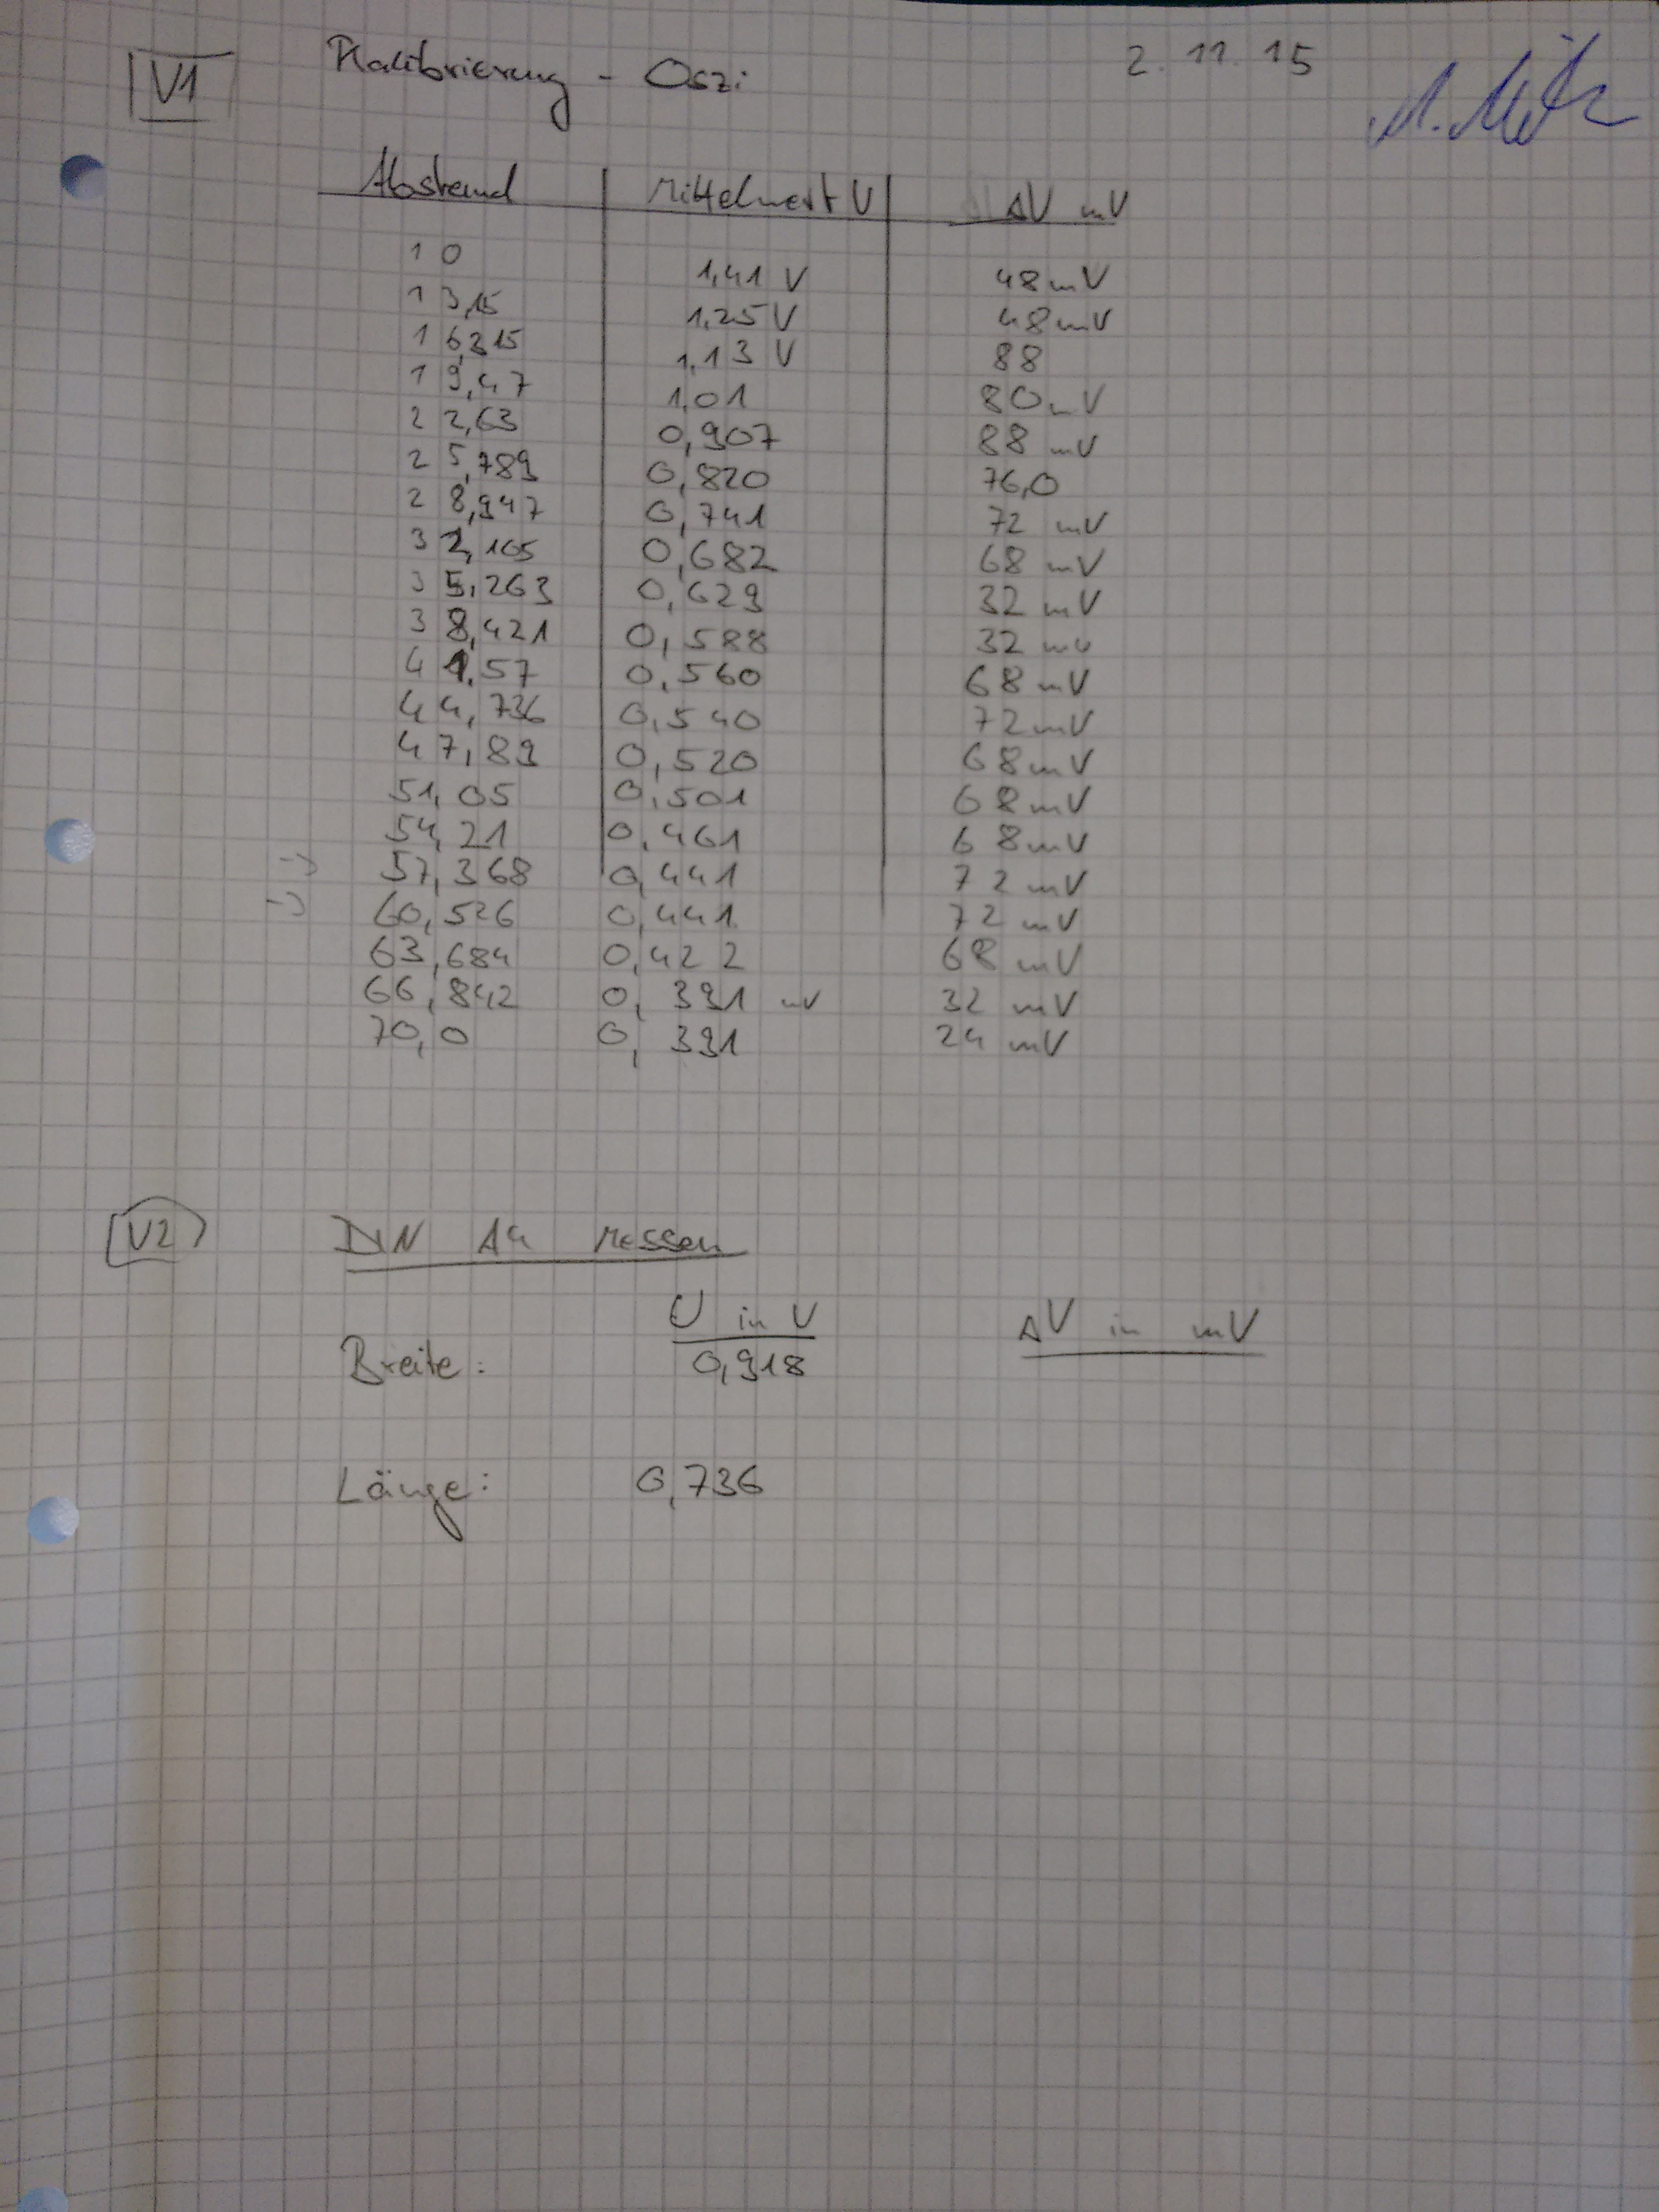
\includegraphics[width=170mm,scale=0.5]{media/MessBlatt.jpg}
	\caption{Messdatenblatt}
	\label{img:MessBlatt}
\end{figure}

%
% Literaturverzeichnis
%
%
% Literaturverzeichnis
%
\phantomsection
\addcontentsline{toc}{chapter}{Literaturverzeichnis}
\bibliography{references}
\newpage

\end{document}
%------------------------------------
% ╔═╗╔╗╔╔╦╗  ╔╦╗╔═╗╔═╗╦ ╦╔╦╗╔═╗╔╗╔╔╦╗
% ║╣ ║║║ ║║   ║║║ ║║  ║ ║║║║║╣ ║║║ ║ 
% ╚═╝╝╚╝═╩╝  ═╩╝╚═╝╚═╝╚═╝╩ ╩╚═╝╝╚╝ ╩ 
%------------------------------------